\section{Algorithm}

\subsection{Feedforward Network Architecture}

The feedforward neural network (FFN) has three layers:
\begin{itemize}
  \item Input layer
  \item Hidden layer
  \item Output layer
\end{itemize}

A graphic view of the FFN can be seen in the following figure:
\pagestyle{empty}

\def\layersep{2.5cm}
\begin{center}
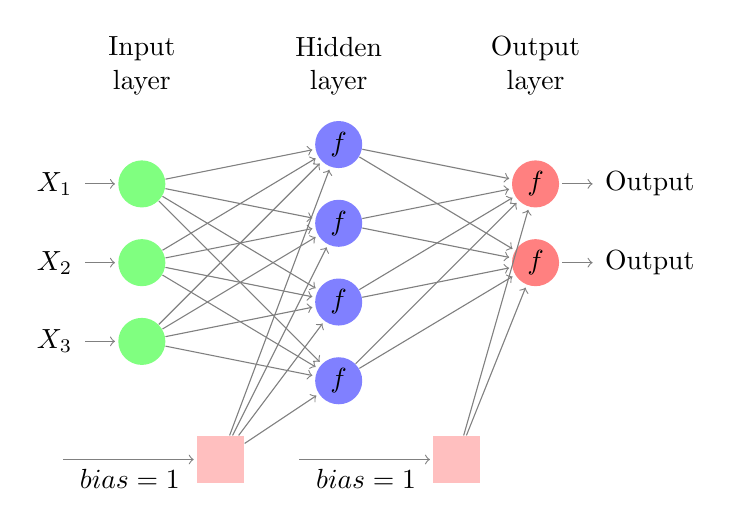
\begin{tikzpicture}[shorten >=1pt,->,draw=black!50, node distance=\layersep]
    \tikzstyle{every pin edge}=[<-,shorten <=1pt]
    \tikzstyle{neuron}=[circle,fill=black!25,minimum size=17pt,inner sep=0pt]
    \tikzstyle{bias}=[rectangle,fill=red!25,minimum size=17pt,inner sep=0pt]
    \tikzstyle{input neuron}=[neuron, fill=green!50];
    \tikzstyle{output neuron}=[neuron, fill=red!50];
    \tikzstyle{hidden neuron}=[neuron, fill=blue!50];
    \tikzstyle{annot} = [text width=4em, text centered]

    % Draw the input layer nodes
    \foreach \name / \y in {1,...,3}
    % This is the same as writing \foreach \name / \y in {1/1,2/2,3/3,4/4}
        \node[input neuron, pin=left:$X_{\y}$] (I-\name) at (0,-\y) {};

    % Draw the hidden layer nodes
    \foreach \name / \y in {1,...,4}
        \path[yshift=0.5cm]
            node[hidden neuron] (H-\name) at (\layersep,-\y cm) {$f$};

    % Draw the output layer node
    \foreach \name / \y in {1,2}
        \node[output neuron, pin={[pin edge={->}]right:Output},right of=H-2] (O-\name) at (2.5,-\y) {$f$};

    % Connect every node in the input layer with every node in the
    % hidden layer.
    \foreach \source in {1,...,3}
        \foreach \dest in {1,...,4}
            \path (I-\source) edge (H-\dest);

    % Connect every node in the hidden layer with the output layer
    \foreach \source in {1,...,4}
        \path (H-\source) edge (O-1);
    \foreach \source in {1,...,4}
        \path (H-\source) edge (O-2);

    % Annotate the layers
    \node[annot,above of=H-1, node distance=1cm] (hl) {Hidden layer};
    \node[annot,left of=hl] {Input layer};
    \node[annot,right of=hl] {Output layer};

    %new bias diagram
    \node[bias] (B-1) at (1,-4.5) {};
    \node[bias] (B-2) at (4,-4.5) {};

    \foreach \hidden in {1,...,4}
        \path (B-1) edge (H-\hidden);
    \foreach \hidden in {1,2}
        \path (B-2) edge (O-\hidden);

    \path[->] (-1,-4.5) edge node [below] {$bias=1$} (B-1);
    \path[->] (2,-4.5) edge node [below] {$bias=1$} (B-2);

\end{tikzpicture}
\end{center}


Each layer of the FFN has several neurons.
The input $\eta_{i}$ of every hidden neuron $i$ will be:
\[
  \eta_{i} =
  f\left(
    \sum_{j=1}^{n}
    w_{i,j}\,x_j + bias_{i,1}
  \right),
\]
where $w_{i,j}$ is the weight
between the hidden neuron $i$ and the input $x_j$.
The function $f$ is the activation function.

The input $\gamma_{i}$ of every output neuron $i$ will be:
\[
  \gamma_{i} =
  f\left(
    \sum_{j=1}^{h}
    \delta_{i,j}\,\eta_i + bias_{i,2}
  \right),
\]
where $\delta_{i,j}$ is the weight
between the output neuron $i$ and hidden neuron output $j$.

To simplify the operations, the connections have been represented by two matrices:

\begin{description}
 \item[W:]
   This matrix stores all the weights between the input and the hidden neurons, i.e.
   $w_{i,j}$ is the weight between the hidden neuron $i$ and the input neuron $j$

  \[
    W_{h \times {n+1}} =
    \left[
      \begin{array}{ccc|c}
        w_{1, 1} & \cdots & w_{1, n} & w_{1, n+1} \\
        \vdots   & \ddots & \vdots   & \vdots     \\
        w_{h, 1} & \cdots & w_{h, n} & w_{h, n+1}
      \end{array}
    \right],
  \]
  where $h$ the total number of hidden neurons,
  $n$ is the number of inputs (number of features)
  and the last column has the bias of every hidden neuron.

 \item[$\Delta$:] This matrix represent the weights between the input and the hidden layer, i.e.
  $\delta_{i,j}$ is the weight between the output neuron $i$ and the hidden neuron $j$

  \[
    \Delta_{m \times h+1} =
    \left[
      \begin{array}{ccc|c}
        \delta_{1,1} & \cdots & \delta_{1,h} & \delta_{1,h+1}\\
        \vdots & \ddots &  \vdots & \vdots\\
        \delta_{m,1} & \cdots & \delta_{m,h} &\delta_{m,h+1}
      \end{array}
    \right],
  \]
  where $m$ is the number of outputs,
  $h$ the total number of hidden neurons
  and the last column has the bias of every hidden neuron.

\end{description}


\subsection*{Activation function}

All the neurons of the same layer have the same activation function $\Phi$.
The hidden layer will always have the logistic sigmoid function:
\[
  \Phi(x) = \frac{1}{1 + e^{-x}}
\]

However, the output layer will depend of the expected output of the problem.
\[
  \Phi(x) =
  \begin{cases}
     \text{Probability} & \frac{1}{1 + e^{-x}} \\
     \text{Real number} & x
  \end{cases}
\]


\subsection*{Procedure}

The output of the FFN is obtained
using a matricial representation of the problem.
The input of the problem is a vector with $n$ features:
\[
  X =
  \begin{bmatrix}
    x_1    \\
    \vdots \\
    x_n    \\
    1
  \end{bmatrix}
\]

In order to simplify the implementation, a feature with value $1$ is added at the end of the vector.

The following steps explain in detail our implementation:

\begin{description}
  \item[Step 1:]
    To calculate the input of every hidden neuron,
    is necessary to get the linear combination between weights and inputs, i.e:
    \[
      \eta_{i} = \sum_{j=1}^{n+1} w_{i,j}\,x_j
    \]
    If we do that using matrices we will have:
    \[
      H =
      \begin{bmatrix}
        \eta_1 \\
        \vdots \\
        \eta_h
      \end{bmatrix} =
        W_{h \times{n+1} } =
        \left[
          \begin{array}{ccc|c}
            w_{1, 1} & \cdots & w_{1, n} & w_{1, n+1} \\
            \vdots   & \ddots & \vdots   & \vdots     \\
            w_{h, 1} & \cdots & w_{h, n} & w_{h, n+1}
          \end{array}
        \right]
        \times
        \begin{bmatrix}
          x_1    \\
          \vdots \\
          x_n    \\
          1
        \end{bmatrix}
    \]

  \item[Step 2:]
    To apply the activation function to every hidden neuron,
    the function must be applied to every component of $H$:
    \[
      H =
      \begin{bmatrix}
        \Phi(\eta_1) \\
        \vdots       \\
        \Phi(\eta_h)
      \end{bmatrix}
    \]

  \item[Step 3:]
    In order to add the bias in the output layer
    it is necessary to add a new component
    with value $1$ to the $H$ vector:
    \[
      H =
      \begin{bmatrix}
        \eta_1 \\
        \vdots \\
        \eta_h \\
        1
      \end{bmatrix}
    \]

  \item[Step 3:]
    To calculate the input of every output neuron,
    is necessary to get the linear combination
    between the weights of connection between the output
    and hidden layer $\Delta$ and the vector $H$ obtained in the step 2, lets define:
    \[
      \gamma_{i} =
      \sum_{j=1}^{h}
      \delta_{i,j}\,\eta_j
    \]
    Using matrices the representation is the following:
    \[
      \Gamma =
      \begin{bmatrix}
        \gamma_1 \\
        \vdots   \\
        \gamma_m
      \end{bmatrix}
      =
      \left[
        \begin{array}{ccc|c}
          \delta_{1,1} & \cdots & \delta_{1,h} & \delta_{1,h+1} \\
          \vdots       & \ddots & \vdots       & \vdots         \\
          \delta_{m,1} & \cdots & \delta_{m,h} &\delta_{m,h+1}
        \end{array}
      \right]
      \times
      \begin{bmatrix}
        \eta_1 \\
        \vdots \\
        \eta_h \\
        1
      \end{bmatrix}
    \]

  \item[Step 4:]
    To apply the activation function of every output neuron,
    the function must be applied to every component of $\Gamma$:
    \[
      \Gamma=
      \begin{bmatrix}
        \Phi(\gamma_1) \\
        \vdots         \\
        \Phi(\gamma_m)
      \end{bmatrix}
    \]
    The vector $\Gamma$ correspond to the output we are looking for.

\end{description}


\subsection*{Pseudocode}
The algorithm \ref{alg:ffn} shows the representation of the problem using matrices.
This algorithm is executed for each arriving input vector.

\begin{algorithm}
  \caption{Get Output of FFN}
  \begin{algorithmic}
    \label{alg:ffn}
    \REQUIRE X, W, $\Delta$
    \ENSURE $\Gamma$

    \STATE H $\leftarrow$ W $\times$ X
    \STATE H $\leftarrow$ $\Phi$(H)

    \STATE $\Gamma$ $\leftarrow$ $\Delta$ $\times$ H
    \STATE $\Gamma$ $\leftarrow$ $\Phi$($\Gamma$)
  \end{algorithmic}
\end{algorithm}


\section{Weight Matrices}

The matrices needed to run the code are:
\begin{itemize}
 \item Matrix representing weights from hidden to input layer ($W$).
 \item Matrix representing weights from output to hidden layer ($\Delta$)
\end{itemize}

In order to test the application, matrices were randomly generated using the following sizes:
\begin{description}
 \item[n:] The number of features of the vector.
 \item[h:] The number of hidden neurons.
 \item[m:] The number of output neurons.
\end{description}


\subsection*{Format}

Matrix $W$, which has $h$ rows and $n+1$ columns, must be saved in a plain text file,
where each line contains the values of a row, separated by spaces.
For example, if the network has $2$ input neurons and $3$ hidden neurons, the file containing matrix $W$
could be formatted as follows:
\begin{verbatim}
-0.2453 0.0951 0.87
-0.0173 0.1471 -0.2
0.9205 -0.0710 0.3
\end{verbatim}
Where the last column correspond to the bias of every hidden neuron.

Matrix $\Delta$, which has $m$ rows and $h+1$ columns,
must be saved in the same format.
The last column must be the bias of the output layer.

\subsection*{Implementations}

Despite of matrices being represented in tabular format in text files,
these are always stored in memory as a one-dimensional array in row order,
i.e. all the rows of the matrix will be saved adjacently in the array.

